% Capíulo 4
\chapter{Avaliação} \label{ch:avaliacao}

Este capítulo descreve o estudo empírico realizado em dois sistemas \textit{open-source} de diferentes domínios cujo objetivo é avaliar se as visualizações são úteis para representar os desvios de desempenho encontrados durante a análise desses sistemas, além de avaliar a facilidade de se encontrar informações e a possível aplicabilidade da ferramenta como parte integrande dos processos de desenvolvimento dos sistemas analisados.

O restante deste capítulo está organizado como segue: seção \ref{sec:avaliacao-projeto} apresenta como o estudo foi projetado, incluindo as principais contribuições (subseção \ref{subsec:avaliacao-principais-contribuicoes}), os objetivos e questões de pesquisa (subseção \ref{subsec:avaliacao-objetivos-questoes-pesquisa}), os sistemas analisados e os procedimentos do estudo (subseção \ref{subsec:avaliacao-sistemas-procedimentos}); a seção \ref{sec:avaliacao-resultados} exibe os resultados do estudo e a seção \ref{sec:avaliacao-consideracoes} conclui o capítulo, apresentando as ameaças à validade e discussões sobre os resultados.

\section{Projeto} \label{sec:avaliacao-projeto}

O estudo analisou um total de 20 releases dos projetos Jetty \cite{Jetty2016} e VRaptor \cite{VRaptor2017}, sendo 10 releases para cada sistema, considerando 193 cenários distintos ao total, gerando as visualizações de sumarização dos cenários e grafo de chamadas para todos os casos. Sobre as visualizações, foram coletados feedback de usuários desses sistemas através de um questionário online.

De maneira geral, foram aplicadas as fases discutidas no capítulo \ref{ch:pqae}, subseção \ref{subsec:funcionamento-perfminer}, além do procedimento necessário para gerar os dados para as visualizações, conforme descrito na seção \ref{sec:visao-geral-architecture-qa-evolution} do mesmo capítulo. Em suma: (i) primeiro, os casos de testes automatizados (cada um deles representando um cenário) dos sistemas foram executados e monitorados, resultando em múltiplos bancos de dados; (ii) depois, os dados coletados foram comparados, agrupando releases subsequentes para cada sistema; (iii) então, os elementos identificados com desvios de desempenho foram minerados nos seus sistemas de controle de versão, com o intuito de descobrir os \textit{commits} que alteraram esses artefatos; (iv) por fim, foi executado, para cada versão de cada sistema, o procedimento necessário para gerar os dados que dão suporte às visualizações. Após isso, o questionário online foi elaborado e aplicado.

O questionário foi enviado para todos os contribuidores dos sistemas que possuiam endereço de email registrado na página de contribuidores de cada sistema ou na página do seu perfil. Dos contribuidores que receberam o questionário, 16 deles responderam com algum feedback.

\subsection{Principais Contribuições} \label{subsec:avaliacao-principais-contribuicoes}

As principais contribuições desta avaliação são: (i) a identificação visual dos cenários que mais tiveram desvios de desempenho para os sistemas Jetty e VRaptor, a partir da análise de múltiplas releases; (ii) para os mesmos sistemas, a percepção visual do tipo de desvio dos cenários através da análise de múltiplas releases; (iii) a identificação visual das potenciais causas dos desvios de desempenho dos cenários dos sistemas analisados; (iv) ...

{\color{red}CONTINUAR...}

\subsection{Objetivos e Questões de Pesquisa} \label{subsec:avaliacao-objetivos-questoes-pesquisa}

O principal objetivo deste estudo é investigar se a ferramenta \textit{\toolName}, com suas visualizações e propriedades visuais oferecidas, é capaz de representar as evoluções de desempenho dos cenários analisados, se proporciona uma fácil identificação desses desvios pelos usuários e se é útil para as equipes de desenvolvimento dos sistemas analisados. Ao utilizar a ferramenta, os usuários poderão identificar os cenários com desvios de desempenho e, a partir da análise do grafo de chamadas de cada um deles, tomar conhecimento sobre os \textit{commits} dos métodos que possivelmente foram os responsáveis pelo desvio. A partir de então, ações podem ser tomadas pela equipe de desenvolvimento para sanar possíveis problemas no desempenho das aplicações. O estudo foi guiado pelas seguintes questões de pesquisa:

\textbf{QP1. A ferramenta proposta é capaz de exibir representações visuais que fornecem informações sobre os cenários de determinado release de um sistema que tiveram o maior desvio de desempenho dentre os analisados?} Após as análises realizadas nos releases dos sistemas, a expectativa é que a visualização da sumarização de cenários seja capaz de exibir metáforas visuais que permitam aos usuários identificar informações sobre os cenários. É esperado que a complexidade na identificação dessas informações seja baixa através da metáfora visual e interações oferecidas para ajudar os usuários nessa identificação.

\textbf{QP2. A ferramenta proposta é capaz de exibir visualmente, para determinado cenário analisado, os métodos identificados com desvios de desempenho, além dos \textit{commits} que possivelmente causaram esses desvios?} A expectativa é que a visualização do grafo de chamada seja capaz de exibir elementos visuais que permitam aos usuários encontrar as informações sobre os métodos com desvios de desempenho, além das suas possíveis causas. Espera-se, também, que a complexidade de identificação dessas informações seja baixa através das metáforas visuais oferecidas e das interações implementadas. É importante que os usuários tomem conhecimento sobre as modificações no código-fonte que geraram algum impacto no desempenho dos sistemas.

\textbf{QP3. Os usuários dos sistemas analisados veem benefícios ou vantagens de se usar a ferramenta proposta em seus processos de desenvolvimento?} Espera-se, com essa questão de pesquisa, verificar se os usuários dos sistemas analisados utilizariam a ferramenta em seus processos de desenvolvimento. Além disso, outro aspecto interessante é saber em qual momento desse processo os desenvolvedores vislumbram que a ferramenta pode ser usada.

\subsection{Sistemas e Procedimentos} \label{subsec:avaliacao-sistemas-procedimentos}

Neste estudo foram usados dois sistemas \textit{open-source} de diferentes domínios escolhidos através dos seguintes critérios: (i) ser desenvolvido na linguagem de programação Java; (ii) ter no mínimo dez releases; (iii) possuir casos de testes automatizados utilizando a biblioteca JUnit; (iv) estar listado em uma das categorias do site \href{http://java-source.com}{http://java-source.com} (site de projetos \textit{open-source} em Java). Os sistemas foram escolhidos de modo que não houvesse repetição de categorias; (v) possuir repositório no GitHub.

A partir desses critérios, foram escolhidos os sistemas Jetty \cite{Jetty2016} e o VRaptor \cite{VRaptor2017}. O Jetty é um servidor web e um servlet contêiner Java capaz de fornecer conteúdo estático e dinâmico a partir de instanciações \textit{standalone} ou embutidas. As dez últimas releases estáveis do Jetty foram escolhidas no momento do início do estudo. Dessa forma, as versões escolhidas foram 9.3.10, 9.3.11, 9.3.12, 9.3.13, 9.3.14, 9.3.15, 9.3.16, 9.4.0, 9.4.1 e 9.4.2.

O VRaptor é um \textit{framework} MVC para desenvolvimento web em Java que visa trazer alta produtividade para um desenvolvimento com CDI. As dez últimas releases estáveis do VRaptor foram escolhidas no momento do início do estudo. Assim, as versões escolhidas foram 4.0.0.Final, 4.1.0.Final, 4.1.1, 4.1.2, 4.1.3, 4.1.4, 4.2.0.RC1, 4.2.0.RC2, 4.2.0.RC3 e 4.2.0.RC4.

Após a escolha dos sistemas e suas releases, os códigos-fonte de todas elas foram baixadas do repositório com a finalidade de executar as três fases do \textit{\perfMinerName}. Após o download, cada uma das versões foi configurada para compilar e executar sem erros, uma vez que a fase 1 necessita exercitar a aplicação através dos testes automatizados. Todos os testes executados são considerados como pontos de entrada de cenários. Para o cálculo do desvio de desempenho, o \textit{\perfMinerName} não considera quaisquer desvios a partir de classes de teste, somente de classes do código-fonte da aplicação.

Os projetos foram configurados para dar suporte ao \textit{AspectJ} e para incluir as bibliotecas do \textit{\perfMinerName}, no entanto, de maneira não intrusiva, sem qualquer alteração no código-fonte. Após isso, para cada versão de cada sistema, todos os casos de testes automatizados foram executados para que os dados da análise dinâmica fossem coletados pela ferramenta.

A análise dinâmica (fase 1) para todas as releases foi executada no mesmo computador sob as mesmas condições e com serviços não essenciais desabilitados. A configuração do computador utilizado foi um AMD Phenom II com 8 GB de memória RAM, executando o sistema operacional Linux Ubuntu 16.04 LTS e o Java na versão 8. A suite de testes automatizados de cada release foi executada dez vezes nas mesmas condições a fim de obter médias de desempenho, em termos de tempo de execução, mais precisas.

Na sequência, as dez releases de cada sistema foram agrupadas em 9 pares de evoluções para executar as fases 2 e 3 do \textit{\perfMinerName}, além da extensão proposta pelo \textit{\toolName}. As tabelas \ref{tab:summary-jetty} e \ref{tab:summary-vraptor} a seguir mostram como ficaram organizados esses pares para cada sistema.

\begin{table}[!htb]
  \textsf{\caption{Resumo para o Jetty.\label{tab:summary-jetty}}}
  \centering
  \medskip
  \begin{tabular}{c|c|c|c|c}
  \textbf{Versão Inicial} & \textbf{Versão Final} & \textbf{\begin{tabular}[c]{@{}c@{}}Cenários\\ Degradados\end{tabular}} & \textbf{\begin{tabular}[c]{@{}c@{}}Cenários\\ Otimizados\end{tabular}} & \textbf{\begin{tabular}[c]{@{}c@{}}Total de\\ Cenários\end{tabular}} \\ \hline
  9.3.10 & 9.3.11 & 5 (3,18\%) & 1 (0,63\%) & 157 \\ \hline
  9.3.11 & 9.3.12 & 0 (0\%) & 36 (21,55\%) & 167 \\ \hline
  9.3.12 & 9.3.13 & 0 (0\%) & 7 (4,51\%) & 155 \\ \hline
  9.3.13 & 9.3.14 & 0 (0\%) & 0 (0\%) & 157 \\ \hline
  9.3.14 & 9.3.15 & 3 (1,84\%) & 2 (1,22\%) & 163 \\ \hline
  9.3.15 & 9.3.16 & 2 (1,21\%) & 1 (0,60\%) & 165 \\ \hline
  9.3.16 & 9.4.0 & 28 (14,97\%) & 6 (3,20\%) & 187 \\ \hline
  9.4.0 & 9.4.1 & 1 (0,53\%) & 0 (0\%) & 186 \\ \hline
  9.4.1 & 9.4.2 & 4 (2,15\%) & 0 (0\%) & 186 \\ \hline
  \multicolumn{2}{c|}{\textbf{Total}} & 43 & 53 & 1523
  \end{tabular}
\end{table}

\begin{table}[!htb]
  \centering
  \textsf{\caption{Resumo para o VRaptor.\label{tab:summary-vraptor}}}
  \medskip
  \begin{tabular}{c|c|c|c|c}
  \textbf{Versão Inicial} & \textbf{Versão Final} & \textbf{\begin{tabular}[c]{@{}c@{}}Cenários\\ Degradados\end{tabular}} & \textbf{\begin{tabular}[c]{@{}c@{}}Cenários\\ Otimizados\end{tabular}} & \textbf{\begin{tabular}[c]{@{}c@{}}Total de\\ Cenários\end{tabular}} \\ \hline
  4.0.0.Final & 4.1.0.Final & 36 (4,86\%) & 41 (5,54\%) & 740 \\ \hline
  4.1.0.Final & 4.1.1 & 0 (0\%) & 0 (0\%) & 745 \\ \hline
  4.1.1 & 4.1.2 & 20 (2,66\%) & 10 (1,33\%) & 750 \\ \hline
  4.1.2 & 4.1.3 & 9 (1,19\%) & 2 (0,26\%) & 752 \\ \hline
  4.1.3 & 4.1.4 & 0 (0\%) & 0 (0\%) & 739 \\ \hline
  4.1.4 & 4.2.0.RC1 & 0 (0\%) & 1 (0,12\%) & 774 \\ \hline
  4.2.0.RC1 & 4.2.0.RC2 & 4 (0,51\%) & 1 (0,12\%) & 776 \\ \hline
  4.2.0.RC2 & 4.2.0.RC3 & 6 (0,77\%) & 0 (0\%) & 771 \\ \hline
  4.2.0.RC3 & 4.2.0.RC4 & 15 (1,94\%) & 3 (0,38\%) & 773 \\ \hline
  \multicolumn{2}{c|}{\textbf{Total}} & 90 & 58 & 6820
  \end{tabular}
\end{table}

Na fase 2, o resultado da análise dinâmica para cada par de releases mostrado anteriormente foi recuperado e comparado, entre os pares, com a finalidade de determinar métodos e contrutores com degradação ou otimização de desempenho. Já na fase 3, os elementos com desvios de desempenho foram minerados nos seus sistemas de controle de versão e sistemas de gerenciamento de tarefas. Ao final das 3 fases do \textit{\perfMinerName}, são gerados os artefatos de saída requeridos para o \textit{\toolName}. Vale salientar neste ponto que, embora o \textit{\perfMinerName} relalize a mineração e obtenha o conjunto de tarefas que estão relacionadas com os \textit{commits} que possivelmente foram os responsáveis por inserir determinado desvio de desempenho, a integração com essas ferramentas de gerenciamento de tarefas está, até este momento, fora do escopo do \textit{\perfMinerName}.

Com os artefatos de saída, a fase 4, pertencente à extensão proposta, foi iniciada. Para cada sistema e um par de releases foi executada uma análise, conforme descrito na subseção \ref{subsec:new-analysis}, cuja finalidade é, a partir desses artefatos, realizar um processamento com o intuito de gerar os dados que dão suporte às visualizações. Após a execução dessa fase, iniciou-se o processo de verificação das visualizações geradas para, posteriormente, publicar o resultado das análises em um ambiente na nuvem, o Heroku\footnote{\href{http://www.heroku.com}{http://www.heroku.com}}, cujo endereço é \href{http://apvis.herokuapp.com}{http://apvis.herokuapp.com}.

A elaboração do questionário se deu na sequência, após a publicação dos resultados das análises. O questionário foi dividido em 5 seções: (i) uma com questões demográficas, (ii) outra com questões sobre o atributo de qualidade de desempenho, (iii) uma terceira com questões sobre a visualização do grafo de chamadas, (iv) outra sobre a visualização da sumarização de cenários e, por fim, (v) uma seção com questões gerais que concluem o questionário.

Os participantes foram agrupados de acordo com o sistema em que contribui. Sendo assim, dois grupos foram formados: 66 participantes para grupo de contribuidores Jetty e 48 para o grupo de contribuidores do VRaptor. Depois, cada grupo foi dividido em dois, de modo que, para cada sistema, foram aplicados dois tipos de questionários. A tabela \ref{tab:survey-groups} mostra a divisão dos grupos de participantes:

\begin{table}[!htb]
  \centering
  \textsf{\caption{Distribuição dos grupos de participantes.\label{tab:survey-groups}}}
  \medskip
  \begin{tabular}{c|c|c|c|c}
  \textbf{Grupo} & \textbf{Sistema} & \textbf{\begin{tabular}[c]{@{}c@{}}Quantidade\\ de Participantes\end{tabular}} & \textbf{\begin{tabular}[c]{@{}c@{}}Tipo de\\ Questionário\end{tabular}} & \textbf{Idioma} \\ \hline
  A & Jetty & 33 & Tipo 1 & Inglês \\ \hline
  B & Jetty & 33 & Tipo 2 & Inglês \\ \hline
  C & VRaptor & 24 & Tipo 1 & Português \\ \hline
  D & VRaptor & 24 & Tipo 2 & Português \\ \hline
  \end{tabular}
\end{table}

Os tipos dos questionários têm as seguintes características: 

\begin{itemize}
    \item \textit{Tipo 1}: neste tipo o participante respondeu às questões sobre a visualização do grafo de chamadas através da visualização exibida pela ferramenta. Por outro lado, as questões sobre a visualização da sumarização de cenários foram respondidas baseadas em resultados dispostos em uma tabela, ao invés da na visualização propriamente dita;
    \item \textit{Tipo 2}: é o inverso do anterior: o participante respondeu às questões sobre a visualização do grafo de chamadas se baseando em resultados exibidos em uma tabela e respondeu às questões sobre a visualização da sumarização de cenários através da visualização mostrada pela ferramenta.
\end{itemize}

A divisão do questionário nesses dois tipos permite que as respostas sejam comparadas entre os que responderam baseados nas visualizações da ferramenta e os que responderam baseados em dados tabulares. Ambos os tipos tiveram questões iguais, no entanto, utilizando referências específicas aos cenários dos projetos analisados, quando aplicado nas questões. Através dessa divisão, pode ser comparado, por exemplo, o porcentual de acerto às questões com e sem as visualizações. Os dois tipos do questionário podem ser consultados no apêncice \ref{ch:apendice-a}.

Com o questionário elaborado, foram coletados os dados de email e login dos contribuidores de cada projeto através da API do Github. No entanto, não foi possível coletar esses dados para todos os contribuidores pelo fato de existir uma opção nessa ferramenta em que os usuários podem desabilitar a publicização do seu endereço de email nessa API. Para esses casos foram feitas visitas manuais aos perfis de cada contribuidor. Ao final desse processo, foram submetidos 66 questionários para os contribuidores do Jetty e 48 para os contribuidores do VRaptor, um total de 114.

\section{Resultados} \label{sec:avaliacao-resultados}

Nesta seção serão discutidos os resultados obtidos após a execução da ferramenta para os sistemas mencionados e após a aplicação do questionário online com os desenvolvedores dessas aplicações. A subseção \ref{subsec:avaliacao-comportamento-visualizacoes} comenta o comportamento das visualizações para os dados obtidos e a subseção \ref{subsec:avaliacao-questionario-online} apresenta os resultados obtidos após a aplicação do questionário.

\subsection{Comportamento das Visualizações} \label{subsec:avaliacao-comportamento-visualizacoes}

asfsfasf

\subsection{Questionário Online} \label{subsec:avaliacao-questionario-online}

Para os dois sistemas analisados, foram aplicados um total de 114 questionários, um para cada participante: 66 para o Jetty e 48 para o VRaptor. Destes, 16 contribuidores responderam com algum feedback: 9 do Jetty e 7 do VRaptor, uma taxa de resposta de 14,04\%. Das respostas, 3 foram consideradas inválidas, pois: (i) em uma delas, o usuário abriu a ferramenta em um celular, comprometendo as visualizações e, consequentemente, as suas respostas; (ii) outro usuário, ao invés de abrir a ferramenta para responder às questões, as respondeu baseada em uma figura explicativa elaborada para elucidar informações sobre as visualizações; e (iii) o terceiro usuário respondeu apenas as questões demográficas, deixando todas as outras em branco. Portanto, 13 respostas foram consideradas válidas para a análise dos resultados.

A maioria dos participantes que responderam são desenvolvedores (31\%), arquitetos (15\%) e engenheiros (23\%) de software, possuem mais de 5 anos de experiência na linguagem de programação Java (figura \ref{fig:avaliacao-questao-2}) e possuem entre 1 e 10 contribuições no seu projeto (figura \ref{fig:avaliacao-questao-3}). Apesar de alguns participantes não terem contribuído para os projetos nos últimos 12 meses, o fato de serem experientes no desenvolvimento de software em Java podem dar credibilidade às suas respostas.

\begin{figure}[!htb]
  \centering
   \begin{subfigure}{.5\textwidth}
   \centering
   \frame{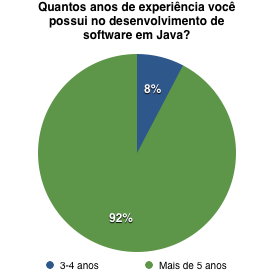
\includegraphics[scale=0.65]{Imagens/avaliacao_questao_2.png}}
   \textsf{\caption[Experiência.]{Experiência em desenvolvimento de software.\label{fig:avaliacao-questao-2}}}
   \end{subfigure}%
   \begin{subfigure}{.5\textwidth}
   \centering
   \frame{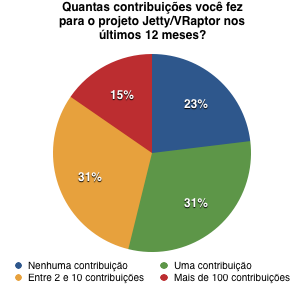
\includegraphics[scale=0.65]{Imagens/avaliacao_questao_3.png}}
   \textsf{\caption[Quantidade de contribuições.]{Quantidade de contribuições.\label{fig:avaliacao-questao-3}}}
   \end{subfigure}
   \caption{Dados demográficos dos participantes.}
  \label{fig:avaliacao-questoes-2-3}
\end{figure}

Sobre a experiência dos participantes com o uso de ferramentas de análise de desempenho, como ferramentas de \textit{profiling} ou ferramentas APM, 54\% declarou usar com frequencia essas ferramentas e 15\% declarou já ter usado pelo menos uma vez. As ferramentas mais citadas pelos participantes foram: JProfiler, New Relic e JVisualVM.

Em resposta à questão \textit{``Suponha que uma funcionalidade do Jetty/VRaptor foi evoluída (por você ou outro membro da equipe). O que você faz para garantir que o tempo de execução/resposta de tal funcionalidade é aceitável em comparação com outras releases?''}, a maioria dos participantes respondeu que fazem a medição de desempenho, no entanto, foram várias as maneiras descritas por eles: o participante P4GA (participante 4 do grupo A) realiza a \textit{``medição e comparação de tempos de execução dos testes''}, já o participante P11GA menciona que faz o \textit{``teste de integração contínua de um teste de gerador de carga''}, o participante P13GC realiza \textit{``análise da complexidade do algoritmo envolvido na evolução e caso não seja possível garantir dessa forma, faço com alguns testes automatizados, seja unitário ou usando um software como o JMeter.''} e o participante P6GD faz \textit{``comparação via NewRelic (response time - response time by endpoint - etc)''}.

\textbf{QP1. A ferramenta proposta é capaz de exibir representações visuais que fornecem informações sobre os cenários de determinado release de um sistema que tiveram o maior desvio de desempenho dentre os analisados?} Os questionários aplicados coletaram dados sobre a utilização da visualização de sumarização de cenários para encontrar informações específicas, bem como da utilização de dados tabulares para encontrar as mesmas informações. Foi observado que...

\textbf{QP2. A ferramenta proposta é capaz de exibir visualmente, para determinado cenário analisado, os métodos identificados com desvios de desempenho, além dos \textit{commits} que possivelmente causaram esses desvios?}

{\color{red}FALTAM MUITAS QUESTÕES AQUI...}

\textbf{QP3. Os usuários dos sistemas analisados veem benefícios ou vantagens de se usar a ferramenta proposta em seus processos de desenvolvimento?} Através do questionário aplicado foi verificado se os participantes veem benefícios na utilização de uma ferramenta como o \textit{\toolName}, além de se eles utilizariam, e de que maneira, a ferramenta em seus processos de desenvolvimento.

Dentre as perguntas dos questionários continha uma específica para os participantes relatarem suas impressões positivas e negativas para cada visualização implementada: \textit{``Você poderia mencionar aspectos dessa visualização que você gostou? E quais outros aspectos você não gostou? Você tem alguma sugestão de melhoria ou comentário para essa visualização?''}. Para a visualização do Grafo de Chamadas, no geral, os participantes disseram gostar das características visuais implementadas, mas também fizeram críticas à visualização. O participante P5GA disse que \textit{``o gráfico é bastante simples e fácil de entender. Não há muita informação, apenas o necessário. Eu gostei do recurso de destaque e a seta verde/vermelha indicando o nível de melhoria/degradação. Como sugestão, pode ser interessante adicionar informações sobre o contexto de execução (ex: argumentos JVM)''}, já o participante P22GA menciona que \textit{``o popup Detalhes é difícil de copiar / colar. Eu preferiria que ele permanecesse aberto até eu clicar em outro lugar. Os links para o commit exato são agradáveis. Toda a visualização parece muito boa, mas gostaria que o grafo de chamadas tivesse um pouco mais de espaço em tela. Seria bom ter (temporariamente?) preenchendo a tela inteira. Por algum motivo, eu esperava poder clicar e arrastar o grafo de chamadas (como o Google Maps) em vez de usar a rolagem.''}. O participante P13GC, no entanto, não percebeu que a funcionalidade de zoom foi implementada e relatou sentir falta: \textit{``gostei dos gráficos e dos detalhes das informações. Achei o espaço reservado para o grafo de chamadas muito reduzido, o espaço vertical pra ele é pequeno. Outra coisa que senti falta foi uma opção de Zoom Out no grafo de chamadas.''}.

Para a visualização da Sumarização de Cenários o sentimento foi dividido. O participante P1GD não se sentiu confortável com o gráfico de rosca utilizado para a visualização: \textit{``gráficos em torta ou semelhantes normalmente querem representar 100\% de algo. Usar a largura versus altura não foi intuitivo pra mim. Talvez separar mesmo em dois gráficos e dar a opção de ordenar ou por um ou por outro.}. Por outro lado, o participante P6GD gostou e comentou que \textit{``utilizar a largura, cor e altura da fatia me pareceu uma boa definição para identificação dos aspectos analisados.''}.

Quando responderam a questão \textit{``Você vê benefícios de usar a ferramenta de visualização de desvios de desempenho apresentada? Se sim, quais?''}, \texttt{63\%} dos participantes disseram que veem benefícios no uso da ferramenta, conforme exibe a figura \ref{fig:avaliacao-questao-16}. Dentre os benefícios comentados pelos participantes, alguns exemplos do que foi informado são: o participante P8GC disse que \textit{``aparentemente pode trazer análises mais assertivas do atual desempenho do sistema''}, o participante P13GC menciona que \textit{``sim, é bem interessante para verificar se os novos releases contém alterações com prejuízos sérios à performance, podendo algumas vezes até detectar algum problema de lógica ou regra de negócio.''}, já o participante P6GD informa que \textit{``sim. É interessante saber de maneira precisa e quantitativa a quantidade e nível de melhorias e degradações entre versões.''}.

\begin{figure}[!htb]
  \centering
  \begin{subfigure}{.50\textwidth}
   \centering
   \frame{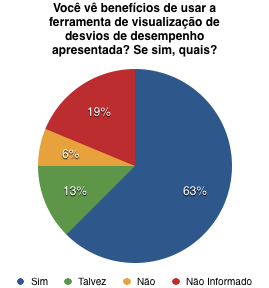
\includegraphics[scale=0.65]{Imagens/avaliacao_questao_16.png}}
   \textsf{\caption[Benefícios da ferramenta.]{Benefícios da ferramenta.\label{fig:avaliacao-questao-16}}}
   \end{subfigure}%
   \begin{subfigure}{.50\textwidth}
   \centering
   \frame{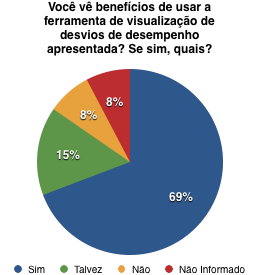
\includegraphics[scale=0.65]{Imagens/avaliacao_questao_17.png}}
   \textsf{\caption[Utilidade da ferramenta.]{Utilidade da ferramenta.\label{fig:avaliacao-questao-17}}}
   \end{subfigure}
   \caption{Questões sobre os benefícios e utilidades da ferramenta proposta.}
  \label{fig:avaliacao-questoes-16-17}
\end{figure}

Com relação à questão \textit{``Você utilizaria a ferramenta como parte integrante do processo de desenvolvimento de software do Jetty/VRaptor? Se sim, como você vislumbra que ela seria utilizada?''}, metade (\texttt{50\%}) dos participantes respondeu que usaria a ferramenta como parte integrante do processo de desenvolvimento. O participante P22GA disse que \textit{``eu imagino usar esta ferramenta de duas maneiras: monitoramento regular para ver como as mudanças afetam o desempenho e investigação focada em uma questão específica.''}, já o participante P8GC reforça que \textit{``talvez ela pudesse fazer parte do conjunto de análises antes da release.''}, o participante P13GC afirma que \textit{``Sim. Acho que poderia ser utilizada para avaliar releases antes de serem lançadas, para garantir que não há consequencias graves à performance após as evoluções implementadas.''} e o participante P18GD disse que \textit{``sim. Integrada ao ciclo de entrega continua (acredito que usam travis.ci) para geração de reports (configurado no maven)''}. A figura \ref{fig:avaliacao-questao-17} sumariza as respostas à essa questão.

Vale destacar que \texttt{19\%} responderam talvez à questão do parágrafo anterior. Dentre as justificativas apresentadas por eles, o participante P4GA disse que \textit{``não sei dizer. Não tenho certeza sobre outros testes mais complexos e de integração''} e o participante P19GD comentou que \textit{``não neste momento. Posteriormente poderia fazer parte de uma análise de status do projeto antes de um release''}.

\section{Considerações} \label{sec:avaliacao-consideracoes}